\documentclass{article}
\usepackage[margin=1in]{geometry} % Sets all margins to 1 inch
\usepackage{graphicx} % Required for inserting images
\usepackage{amsmath}

\title{
Decentralized Fusion Planning for Scalability in Distributed Satellite Tracking\\
{\small ASEN 6519: Optimization, Final Project}}
\author{Nolan Stevenson}
\date{} % This removes the date

\begin{document}

\maketitle

\newpage
\section{Introduction and Background}

	The purpose of this project is to develop an optimization algorithm that solves the decentralized fusion planning problem for scalability in distributed satellite tracking. 
    \\Consider the following situation:\\
    \begin{itemize}
        \item You have a network of LEO satellites, about 200+ total satellites. The satellite network must autonomously track targets, about 50+, on the Earth's surface.
        \item The satellite network is seperated into two different types of satellites, sensing and fusion satellites.
        \item The sensing satellites are able to collect measurements on targets using bearings only sensors.
        \item The sensing layer communicates the measurements to the fusion layer, which is responsible for fusing the measurements and tracking the targets, using extended kalman filters and distrbuted fusion algorithms.
        \item The fusion satellites are limited both computationally on the number of target tracks they can handle at a time, and in communication bandwidth between neighboring satellites.
        \item The entire satellite network must be able to autonomously operate to perform target tracking, this includes: tasking, sensing, fusion, communication, and control.
    \end{itemize}

    The following diagram shows the basic structure of the satellite network; a fusion layer, a sensing layer, and objective targets to track.
    \begin{figure}[h]
        \centering
        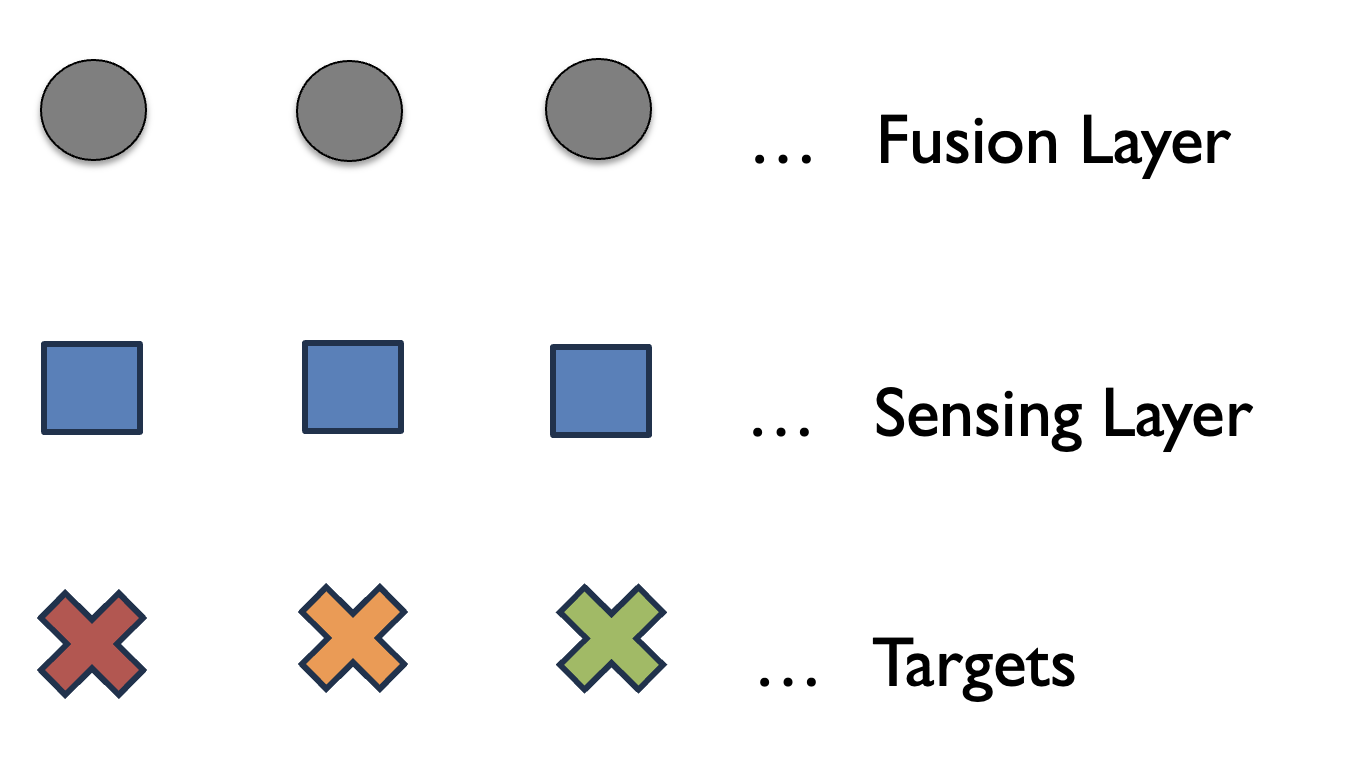
\includegraphics[width=0.5\textwidth]{images/basic_struct.png}
        \caption{Satellite Network Diagram}
        \label{fig:satellite_network}
    \end{figure}

    In order to scalabily track this many targets in a satellite network, it is best to use a technique called "federated tracking". This is a system where each track is essentially treated as a centralized extended kalman filter (EKF). Thus, there is a single fusion node responsible for the EKF of each target.
    However, the challenge with this formulation is deciding which fusion node should be resposible for which target? I will introduce the following terms to help describe the problem:
    \begin{itemize}
        \item \textbf{Custody:} The fusion node that is responsible for the federated EKF for a particular target.
        \item \textbf{Bounty:} The protocol the sensing nodes use to send measurements about a target to the fusion layer.
    \end{itemize}

    With these two terms, there is an algorithm which assigns custody of targets to the fusion nodes. The following diagram represents this algorithm:

    \begin{figure}[h]
        \centering
        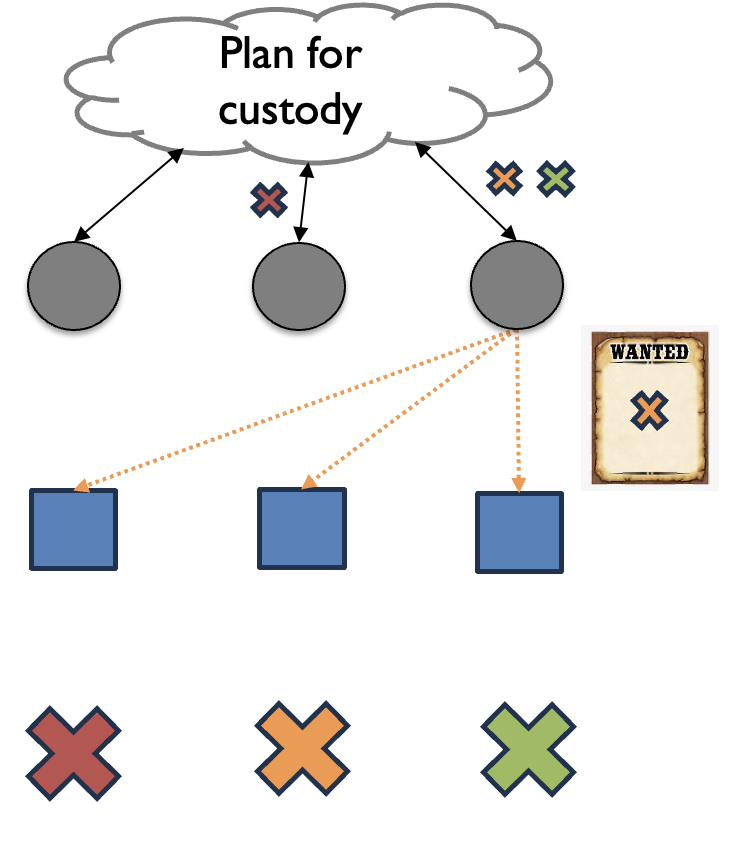
\includegraphics[width=0.4\textwidth]{images/custody_algo.png}
        \caption{Custody Assignment Algorithm}
        \label{fig:custody_algo}
    \end{figure}

    \vspace{4cm} % Adds vertical space after the figure

    This diagram shows the fusion layer nodes having a algorithm that decides who should have "custody" of which targets. The fusion node with custody of a target is responsible for running the "federated/centralized EKF" on that target for the next X amount of time. Once custody is assigned, the fusion nodes send out a "bounty" on that target to the relavent sensing nodes. This bounty essentially says "if you see this target, report back to me". \\
    This is the custody/bounty system I will refer to for the rest of the project. The goal of this project is to develop an optimization algorithm to plan for custody. \\

    The following are goals of the optimization algorithm:
    \begin{itemize}
        \item All targets must be tracked for the next X amount of time.
        \item The computational limit of a fusion node cannot be exceeded (per node, maximum number of EKFs/custody`').
        \item The amount of communication throughout the network should be minimized (not hard limit, computation is limiting factor in this environment).
        \item Whenever the custody of a target is changed, track to track handoff must occur between old owner and new owner.
    \end{itemize}

    \newpage

    \section{Problem Formulation}
    This problem can be formulated as a mixed-integer linear program (MILP), consisting of three key components:
    \begin{enumerate}
        \item Decision variables: These represent the possible choices in the optimization problem.
        \item Objective function: This is the function to be maximized or minimized.
        \item Constraints: These are the limitations or requirements that must be satisfied.
    \end{enumerate}


    The objective function and constraints are expressed in linear combination of the decision variables, creating a mathematical formulation suitable for a linear program solver. In this case, we will use the Python package PuLP, which can efficiently solve MILPs using a branch and bound algorithm.
    
    The problem can be written as: \\
    
    \begin{equation}
        \underset{x_{st}}{\text{minimize}} \sum_{s} \sum_{t} c_{st} x_{st}
        \label{eq:objective}
    \end{equation}
    
    \text{subject to}

    \begin{equation}
        x_{st} \in \{0, 1\} 
        \label{eq:binary}
    \end{equation}

    \begin{equation}
        \sum_{s} x_{st} \geq 1 \quad \forall t
        \label{eq:constraint1}
    \end{equation}

    \begin{equation}
        \sum_{t} x_{st} \leq Comp(s) \quad \forall s
        \label{eq:constraint2}
    \end{equation}

    In the formulation above, $s$ is the index for a fusion satellite, and $t$ is the index for a target. \\
    Equation \eqref{eq:objective} is the objective function, which is to minimize the cost of assigning custodies throughout the network (more dicussion on that cost below). \\
    Equation \eqref{eq:binary} is the binary constraint, which ensures that the decision variable $x_{st}$ is either 0 or 1. If $x_{st} = 1$, then fusion satellite $s$ has custody of target $t$. \\
    Equation \eqref{eq:constraint1} ensures that every target has at least one fusion satellite assigned to it. This means that each target is being tracked in the network. \\
    Equation \eqref{eq:constraint2} ensures that no fusion satellite is assigned more targets than its computational limit, defined as $Comp(s)$. 

    The cost of assigning custody of a target to a fusion satellite is defined as $c_{st}$. A good cost function is one that minimizes the amount of communication throughout the network. 
    Since the goal of the algorithm is to assign custodies for some short horizon into the future, the cost function needs to account for current and future communication needs. 
    A simple choice for the cost function over some planning horizon $T$ is:
    \begin{equation}
        c_{st} = \sum_{k=0}^{T} \| \mathbf{r}_k^{target} - \mathbf{r}_k^s \|
        \label{eq:cost}
    \end{equation}

    The cost function is the sum of the distance between the estimated target position (from the EKF track) and the fusion satellite position (known due to orbit params) over a discrete set of points from current time into the future horizon. This cost function is a good proxy for communication cost because it is a measure of how far the measurement data needs to travel from the sensing satellites to the fusion satellite.

    Thus, this optimization problem is a valid way to plan for custody of targets over some short horizon in the fusion layer without violating computational constraints while minimizing communication costs.
  

    \newpage
    \section{NEW CONTENT AND EQS}

    \begin{equation}
        \sum_{s} x_{st} == \sum_{s} Capacity(s) \quad \forall t
        \label{eq:constraint1}
    \end{equation}

\end{document}